\documentclass{article}
\usepackage[utf8]{inputenc}
\usepackage{tikz}
\usepackage[hidelinks]{hyperref}
\title{Dibujar líneas con TikZ}
\author{Curso de \LaTeX}
\begin{document}
\maketitle

TikZ es un paquete que nos permite crear gráficos directamente desde \LaTeX\ en formatos portable (PGF) de PDF y PostScript.

Este paquete introduce el entorno \texttt{tikzpicture}, el cual podemos utilizar como un lienzo para dibujar nuestros gráficos. Para lograrlo contaremos con un grupo de comandos especiales para dibujar líneas y puntos, siendo el comando \textbackslash\texttt{draw} el más utilizado.

\section*{Líneas rectas}

Las figuras se dibujan por medio rutas (paths). Una ruta es una serie de segmentos de línea recta y curvada. 

Por ejemplo, para dibujar líneas que formen un ángulo recto, utilizamos el comando \textbackslash\texttt{draw} de la siguiente forma:

\begin{tikzpicture}
\draw (1,0) -- (0,0) -- (0,-1);
\end{tikzpicture}

La ruta se dibuja siguiendo una serie de coordenadas que al unirlas con líneas rectas forman la figura. Las coordenadas se introducen en el plano por medio de paréntesis separadas por comas, seguidas de un doble signo de menos que representa las líneas rectas del ángulo. 

Podemos además añadir opciones a cada una de las figuras dibujadas:

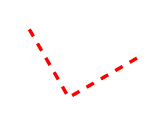
\begin{tikzpicture}
\draw[red, dashed, very thick, rotate=30] (1,0) -- (0,0) -- (0,1);
\end{tikzpicture}

Con estas opciones podemos modificar el color, el estilo y el grosor de las líneas, así como hacer rotar el gráfico en el ángulo que queramos.

Podemos además cerrar los extremos de las líneas con la instrucción ``--cicle'':

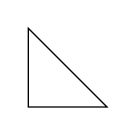
\begin{tikzpicture}
\draw (1,0) -- (0,0) -- (0,1) -- cycle;
\end{tikzpicture}

¡Y obtenemos un triángulo rectángulo!

Las líneas rectas también pueden ser paralelas:

\begin{tikzpicture}
\draw (0,0) -- (2,0) (0,1) -- (2,1);
\end{tikzpicture}

Y combinarse con líneas verticales:

\begin{tikzpicture}
\draw (0,0) -| (1,1);
\end{tikzpicture}

El caracter ``\textbar'' se utiliza para indicar de que lado de la línea se dibujará la vertical, pudiendo también al inicio:

\begin{tikzpicture}
\draw (0,0) |- (1,1);
\end{tikzpicture}

También, podemos modificar la forma de los vértices dibujados:

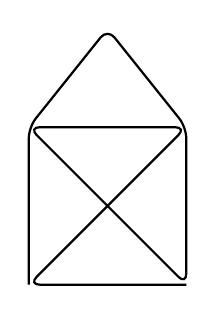
\begin{tikzpicture}
  \draw[thick,rounded corners=4pt] (0,0) -- (0,2) -- (1,3.25) 
   -- (2,2) -- (2,0) -- (0,2) -- (2,2) -- (0,0) -- (2,0);
 \end{tikzpicture}
 
\section*{Curvas}

Se pueden crear líneas curvas con una curva de Bezier\footnote{\url{http://es.wikipedia.org/wiki/Curva\_de\_B\%C3\%A9zier}} con las instrucción ``..controls() ..()'', con uno o dos puntos de control.
 
\begin{tikzpicture}
 \draw (0,0) .. controls (1,1) .. (4,0)
  (5,0) .. controls (6,0) and (6,1) .. (5,2);
\end{tikzpicture}

También podemos crear rutas personalizados utilizando la instrucción ``to''. Si la utilizamos sin ninguna opción se dibujará una línea recta, exactamente igual que el comando doble signo de menos ``--''. Mediante las opciones ``in'' y ``out'' podemos crear un ruta que dibuje un curva. Por ejemplo ``[out = 135, in = 45]'' hace que la ruta salga en un ángulo de 135 grados en la primera coordenada y regrese a un ángulo de 45 grados en la segunda coordenada.

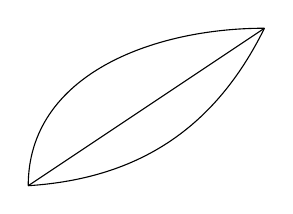
\begin{tikzpicture}
\draw (0,0) to (3,2);
\draw (0,0) to[out=90,in=180] (3,2);
\draw (0,0) to[bend right] (3,2);
\end{tikzpicture}
\end{document}